\documentclass{article}

\usepackage{geometry}
\geometry{margin=2cm}
\usepackage{graphicx}
\usepackage{hyperref}

\hypersetup{colorlinks=true, linkcolor=blue, urlcolor=blue}
\urlstyle{same}
\begin{document}
	
	\author{Aayush Arya}
	\date{(Submitted: \today)}
	\title{}
	
	\maketitle
	
	\hrule
	\begin{center}
		PHY350 Lab Report\\
		Practical No: 2 \quad Registration No.: 11912610 \quad Section: G2903
	\end{center}
	\hrule
	
	\section*{Aim}
	To measure the charge to mass ratio of ...
	
	\section*{Methods}
	We performed the experiment {\it in silico} using a virtual platform\footnote{\url{https://virtuelle-experimente.de/en/b-feld/e-m-bestimmung/edurchm.php}} (see Figure \ref{fig:sim}).
	
	\begin{figure}[h]
		\centering
		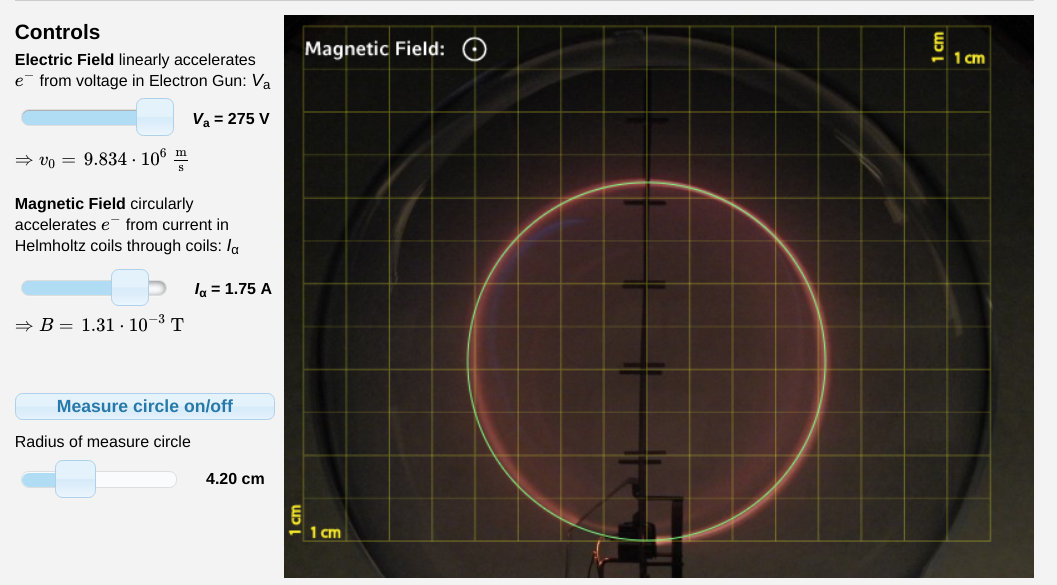
\includegraphics[width=0.8\textwidth]{e_m_ratio}
		\caption{The virtual platform.}
		\label{fig:sim}	
	\end{figure}
	
	\section*{Results}\begin{center}
		
	\end{center}
	The measurements done are summarized below.
	
	\begin{figure}[h]
		\centering
		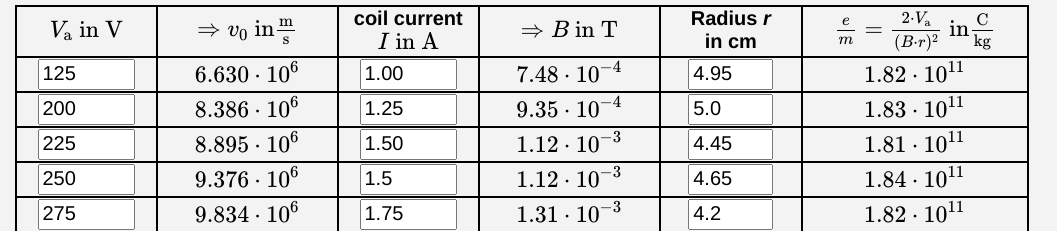
\includegraphics[width=0.7\textwidth]{observations}
	\end{figure}
	
	The mean $e/m$ was found to be $1.82\times10^{11}$ C kg$^{-1}$. This is off the true value of $1.76\times 10^{11}$ by 3.64\%.
	
\end{document}